\documentclass[a4paper, twoside]{report}
\setcounter{tocdepth}{3}
\setcounter{secnumdepth}{3}
%Language and font encodings
\usepackage[english]{babel}
\usepackage[utf8]{inputenc}

\usepackage{titlesec}
\titleformat{\chapter}[display]
  {\Huge\bfseries}
  {}
  {0pt}
  {\thechapter.\ }

\titleformat{name=\chapter,numberless}[display]
  {\Huge\bfseries}
  {}
  {0pt}
  {}

%Sets page size and margins
\usepackage[a4paper,top=3cm,bottom=2cm,left=3cm,right=3cm,marginparwidth=1.75cm]{geometry}

%Useful packages
\usepackage{array}
\usepackage{amsmath}
\usepackage{amssymb}
\usepackage{url}
\usepackage{listings}
\usepackage{color}
\usepackage{longtable}
\usepackage{graphicx}
\usepackage{pdfpages}
\usepackage{enumitem}
\usepackage[hidelinks]{hyperref}
\usepackage{siunitx}
\usepackage{pdfpages}

\title{A Visual GUI Tool for Auto-adjusting Text in Selected Image}

\begin{document}
\begin{titlepage}

\newcommand{\HRule}{\rule{\linewidth}{0.3mm}} % Defines a new command for the horizontal lines, change thickness here


\center % Center everything on the page

\includegraphics[width=9cm]{title/logo.png}\\[1.5cm]

%	TITLE SECTION

\makeatletter
\HRule \\[0.8cm]
{ \huge \bfseries \@title}\\[0.4cm] % Title of your document
\HRule \\[0.5cm]

%	HEADING SECTIONS

\textsc{\Large Ravensburg-Weingarten University}\\[0.3cm] 
\textsc{\large Electrical Engineering and Information Technology}\\ [1.5cm]


\large Bachelor Project Report  \large\\
\textbf{Period:} 01.07.2020 - 30.09.2020\large\


%	AUTHOR SECTION

\vspace{2.5cm}

\begin{minipage}{0.4\textwidth}
\begin{flushleft} \large
\emph{Supervisor:} \\ Prof. Dr. Markus \textsc{Pfeil} 
\end{flushleft}
\end{minipage}
~
\begin{minipage}{0.4\textwidth}
\begin{flushright}\large
\emph{Author and Matrikel-Nr.:}\\ 
Siyi \textsc{Dai} 29245\\
Daniel \textsc{Heimman} 29405 \\

\end{flushright}
\end{minipage}\\[2cm]

\makeatother
%	DATE SECTION

{\large \today}\\[7cm] 



\vfill % Fill the rest of the page with whitespace

\end{titlepage}




\newpage
\tableofcontents
\newpage

\chapter{Introduction}
\section{Definition of Tasks}
\noindent The project tasks are focused on developing graphical user interfaces (GUI) for auto-adjusting text to mouse selected area inside of an image using PyQt5.  \\ \par

\noindent GUI is a form of user interface that allows users to interact with electronic devices through graphical icons, instead of text-based user interfaces, typed command labels or text navigation.  \\ \par

\noindent The text itself should be able to modified with different fonts and sizes, and it should be equipped with wrapping function based on the content.
 \\ \par
 
\noindent The space occupied by the input text should be evaluated and compared with the area the user set with mouse. If the text is overflowed out of the bounding box selected, the user should be able to choose to ignore it or clear the content.  \\ \par


\chapter{Environment Specification}
\noindent The work environment is composed of two sides. The hardware environment which presents the machines or components being used while running code. The software environment which represents the advanced programming interfaces, integrated development environments, editors, technologies and tools being used.  \\ \par

\section{Hardware Environment}
\noindent The table describes the used computer for work while two BenQ Corporation 32" monitors were used. \\ \par

\begin{table}[h]
\centering
\begin{tabular}{|c|c|}
\hline
PC & HP ZBook 15 G5 (3AX13AV) \\
\hline
CPU & Intel(R) Core(TM) i7-8850H CPU @ 2.60GHz \\
\hline
RAM & 32GB \\
\hline
OS & Ubuntu 18.04.3 LTS \\
\hline
Graphics Card & NVIDIA Quadro P1000 Mobile\\
\hline
\end{tabular}
\caption{Characteristics of used computer}
\end{table}


\section{Software Environment}
\paragraph{Python 3.6.10 :: Anaconda, Inc.}
\textit{Python} is an interpreted, high-level, general-purpose programming language. The internship tasks are all coded in \textit{Python 3.6.10} within help of \textit{Anaconda}, which is a \textit{Python} and \textit{R} distribution including the core python language, 100+ Python libraries and package manager \textit{conda}. \\ \par

\paragraph{Visual Studio Code}
\textit{Visual Studio Code} is a free source-code editor  made by \textit{Microsoft} for \textit{Windows}, \textit{Linux}, \textit{macOS}. Features include support for debugging, syntax highlighting, intelligent code completion, snippets, code refactoring, and embedded Git.  \\ \par

\paragraph{PyQt5}
\textit{PyQt5} is a GUI develop application provided by \textit{Python}. It is cross-platform GUI toolkit, a set of python bindings for \textit{Qt v5}. An interactive desktop application can be developed with much easier because of the tools and simplicity provided by this library. \\ \par

\newpage
\noindent \textsc{Modules and Classes: } While the designation of Exporter and Visualizer, various modules and classes from \textit{PyQt5} have been used.   \\ \par
{\renewcommand{\arraystretch}{1.5}%
\begin{table}[h!]
\centering
\begin{tabular}{ m{2cm}| m{.8\textwidth}  }
Modules & Classes \\
\hline
\textit{QtOpenGL} & \textit{QGLFormat} \\
\hline
\textit{QtCore} &\textit{pyqtSignal, Qt, QPoint, QRectF, QSize} \\
\hline
\textit{Qtgui} &\textit{QPainter, QColor, QBrush, QWheelEvent, QPixmap, QMouseEvent, QFont, QFontMetrics} \\
\hline
\textit{QtWidgets} & \textit{QGraphicsView, QGraphicsScene, QGraphicsPixmapItem, QAbstractScrollArea, QGraphicsRectItem, QGraphicsTextItem, QDesktopWidget, QMessageBox, QVBoxLayout, QFileDialog} \\
\end{tabular}
\caption{Modules and Classes being used for developing UI tools}
\end{table} \quad

\paragraph{Qt Creator}
\textit{Qt Creator} includes a code editor and integrates \textit{Qt Designer} for designing and building GUIs from \textit{Qt widgets}. After layout designing and objects naming in \textit{Qt Creator}, a form implementation could be generated from reading ui file by \textit{PyQt5 UI code generator 5.9.2}. \\ \par

\begin{figure}[h!]
\centering
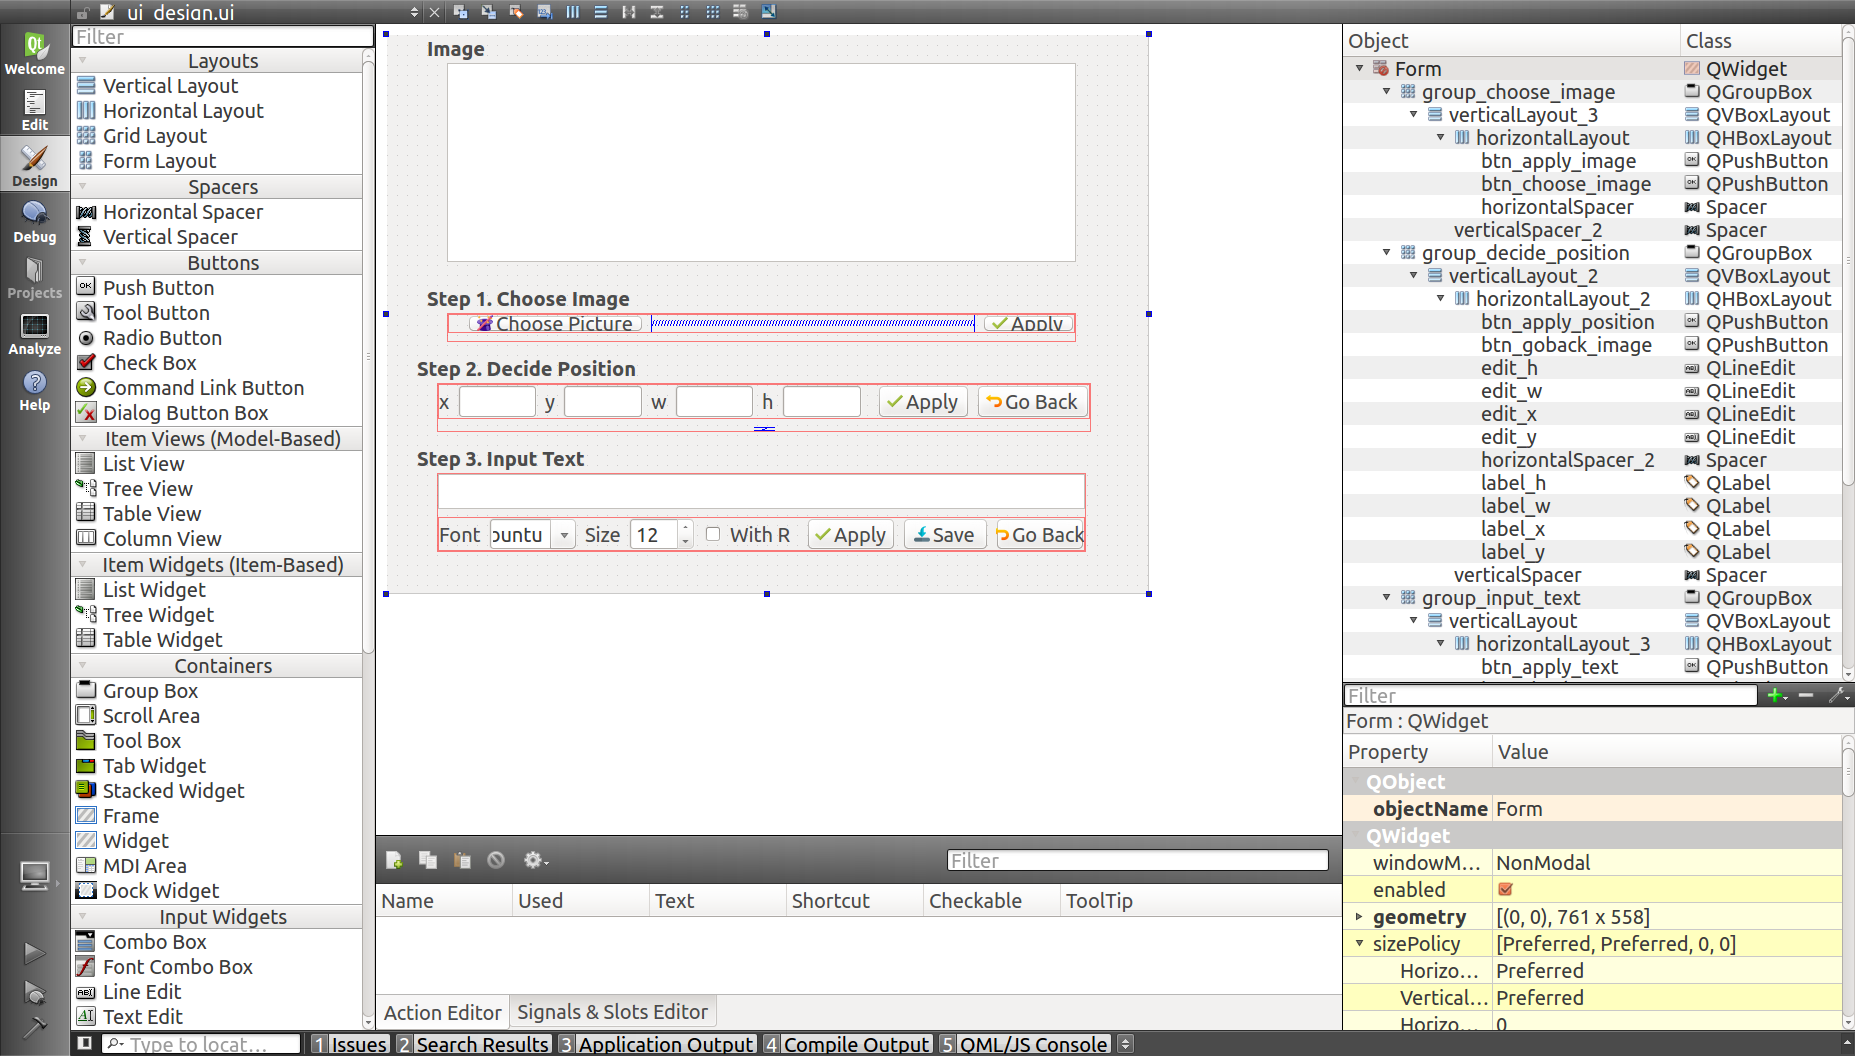
\includegraphics[width=.9\textwidth]{qt_creator.png}
\caption{Qt Creator window in the design frame}
\end{figure}

\chapter{Instruction}
\begin{itemize}

\begin{figure}[h!]
\centering
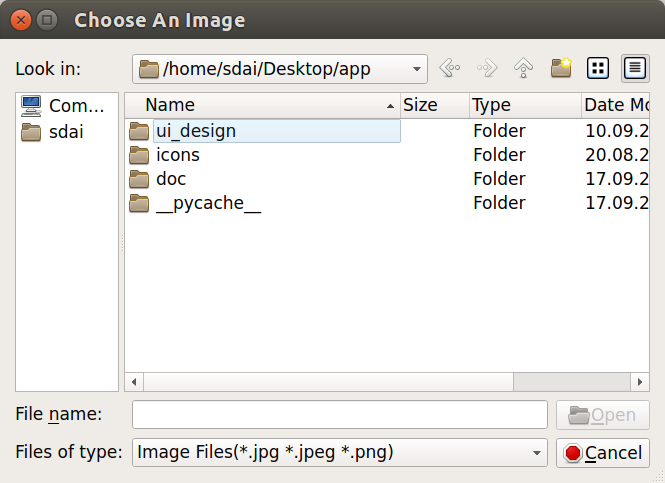
\includegraphics[width=.7\textwidth]{image_choose.png}
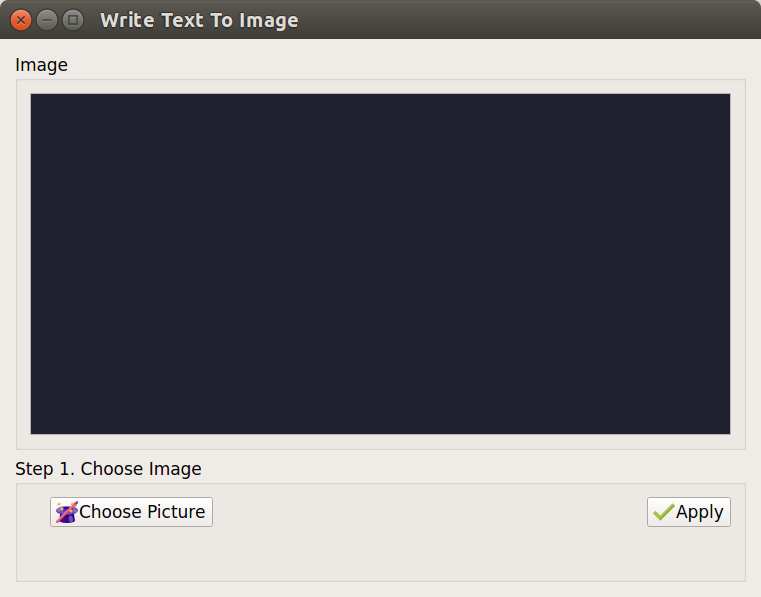
\includegraphics[width=.45\textwidth]{mainwindow.png}
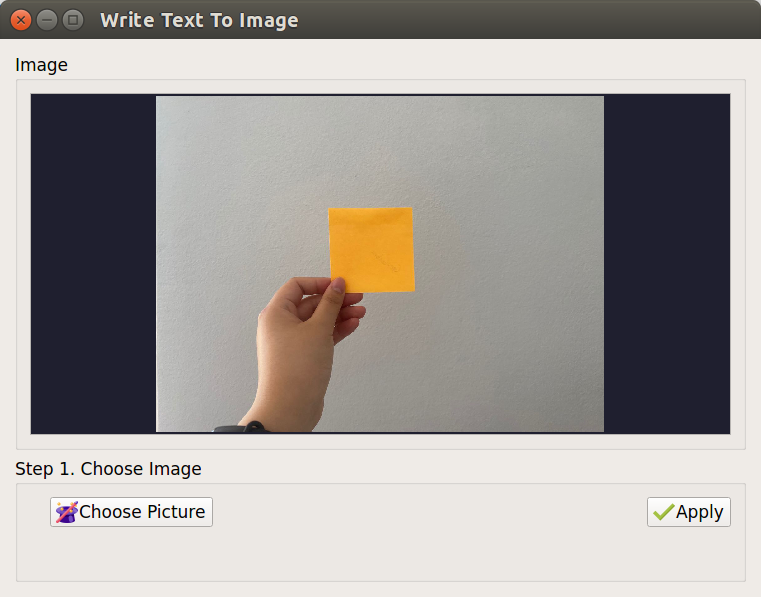
\includegraphics[width=.45\textwidth]{loaded.png}
\caption{Selecting the picture to put text on}
\end{figure}

\item \textbf{Step 1: } After the user selects a picture, click the Apply button and then go to step 2;

\newpage
\begin{figure}[h!]
\centering
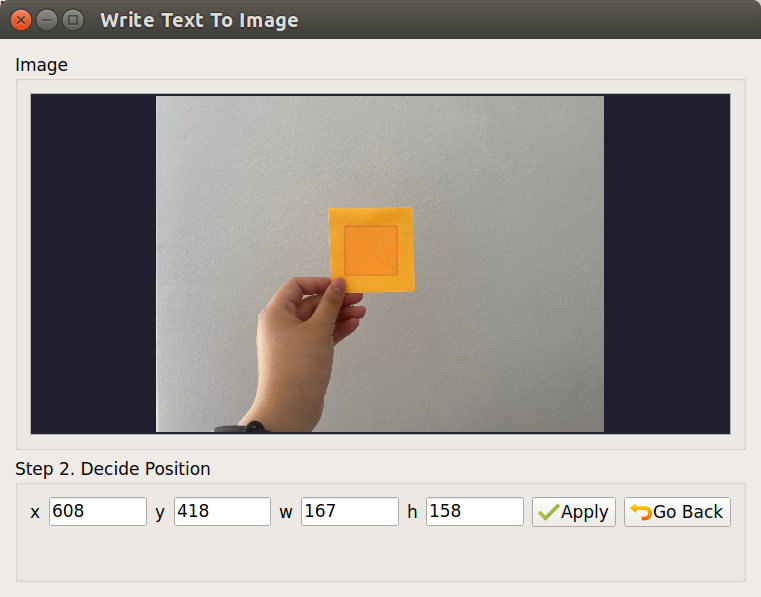
\includegraphics[width=.9\textwidth]{area_select.png}
\caption{Selecting the text area in the image}
\end{figure}

\item \textbf{Step 2: } The user selects the text block with the left mouse button, clicks Apply to enter step 3, and clicks the Go Back button to return to step 1;


\begin{figure}[h!]
\centering
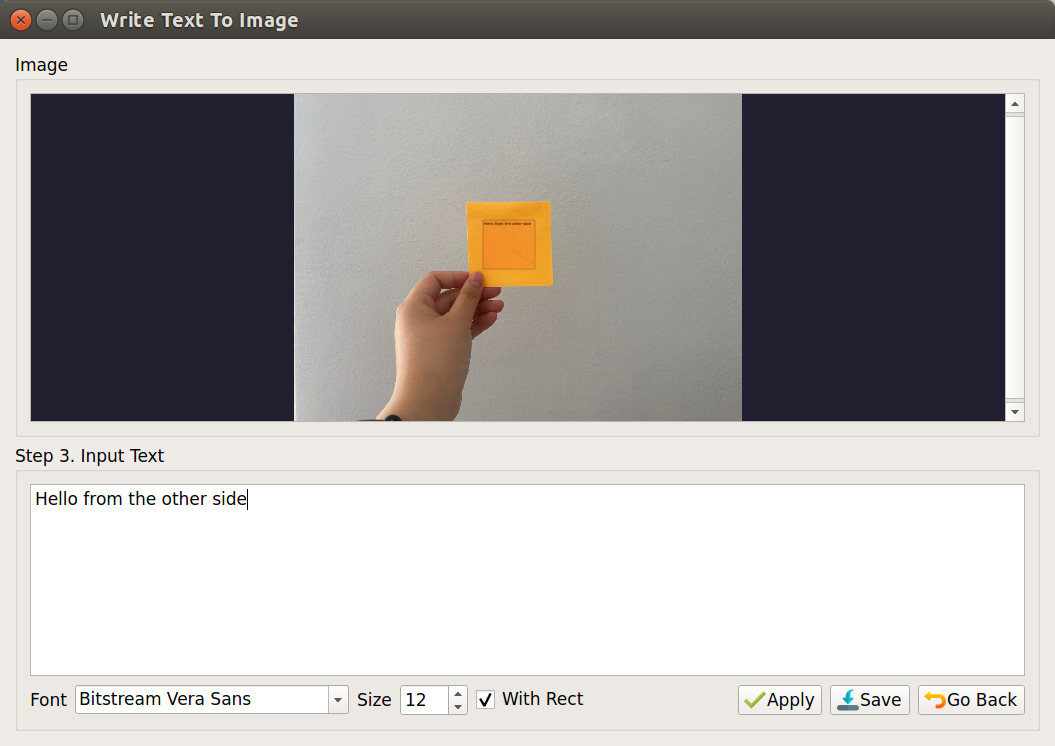
\includegraphics[width=.9\textwidth]{text.png}
\caption{Input the text without font and size modified}
\end{figure}
\item \textbf{Step 3:} The user can enter the text in the groupbox here.

\newpage
\item \textbf{Step 4:} After the user enters the text, select the desired font and font size and click the Apply button. The program will try to place the text in the specified block. The user can click the Go Back button to return to step 2.



\begin{figure}[h!]
\centering
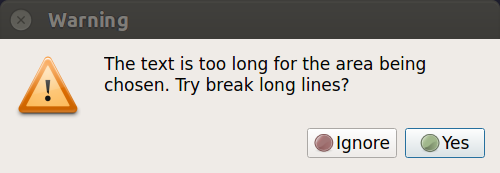
\includegraphics[width=.5\textwidth]{big.png}
\caption{Message box asking for whether break the long lines}
\end{figure}

\noindent If the text is too long for the chosen area, a message box asking for whether break long lines will appear. Once the user clicked Yes, the text will be wrap into several lines.  \\ \par

\begin{figure}[h!]
\centering
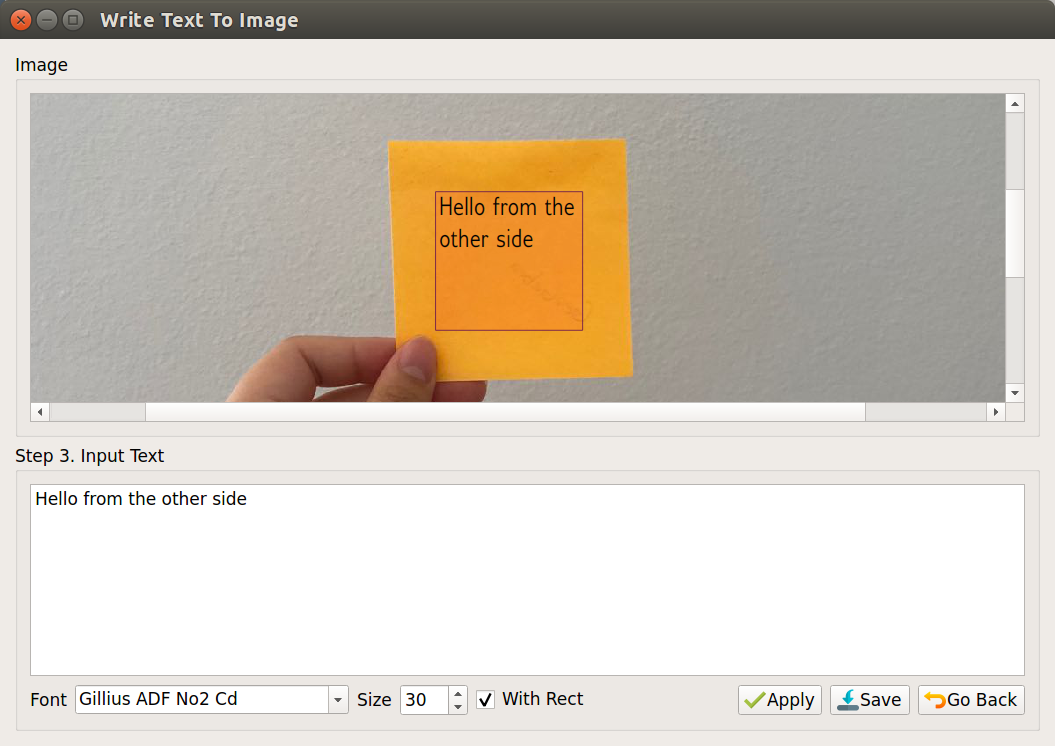
\includegraphics[width=.9\textwidth]{font.png}
\caption{The text modified and wrapped into several lines}
\end{figure}

\newpage
\begin{figure}[h!]
\centering
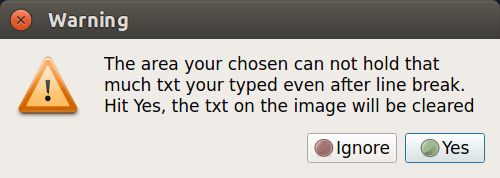
\includegraphics[width=.5\textwidth]{big2.png}
\caption{Message box asking for whether ignore the overflow or clear the content}
\end{figure}


\noindent If the text is still too much for the chosen area even after line wrap, a message box asking for whether ignore the overflow or clear the content will appear. Once the user clicked Yes, the text will be cleared out. Otherwise it will show the overflowed text.   \\ \par

\begin{figure}[h!]
\centering
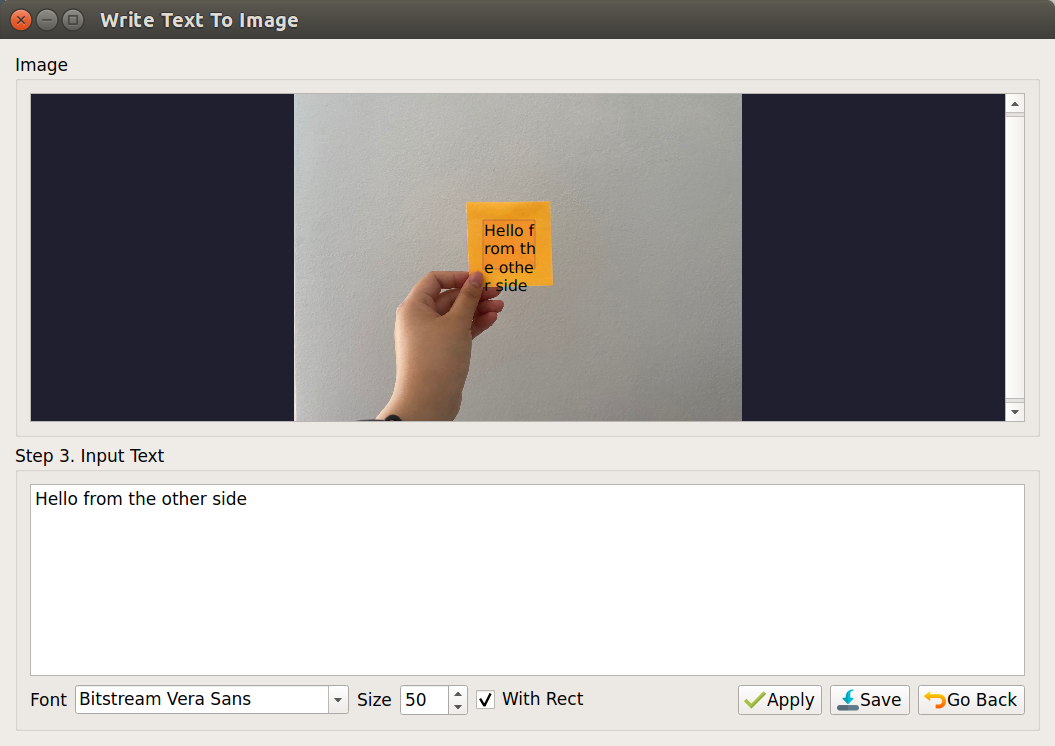
\includegraphics[width=.9\textwidth]{ignore.png}
\caption{Overflowed text}
\end{figure}

\item \textbf{Step 5:} The user can also click the Save button to save The picture containing the text is saved as a png format file. In addition, a selection button is provided, and the user can choose whether to display the text box.

\begin{figure}[h!]
\centering
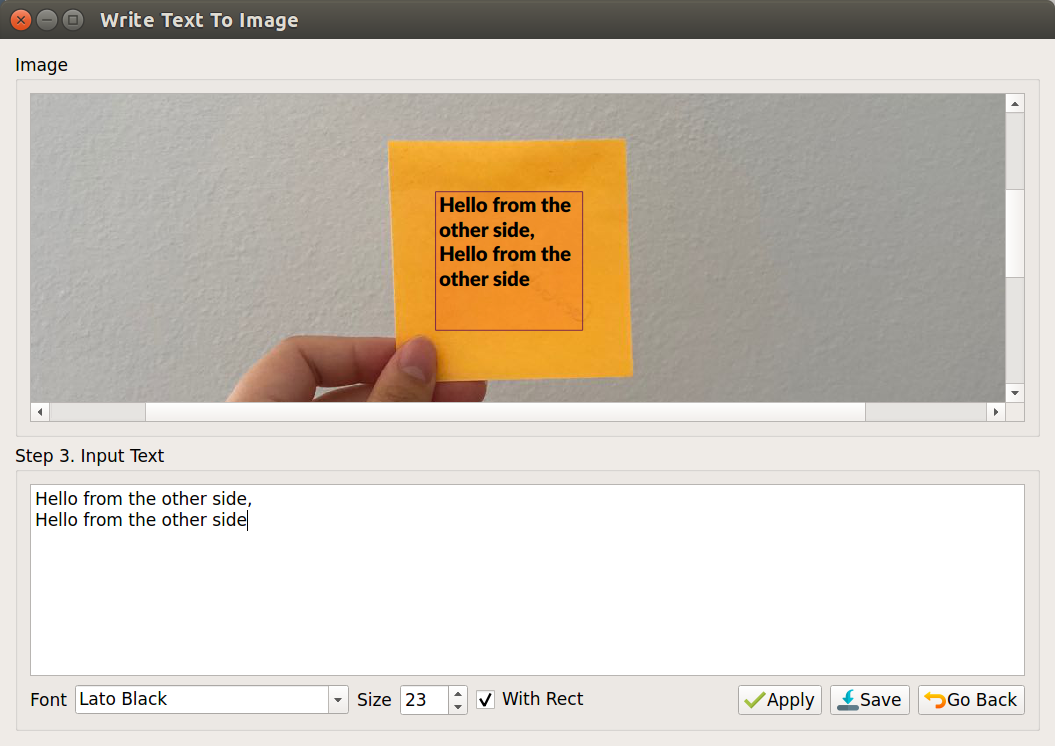
\includegraphics[width=.9\textwidth]{two.png}
\caption{Modify the font and size to fit the text into the chosen area}
\end{figure}

\begin{figure}[h!]
\centering
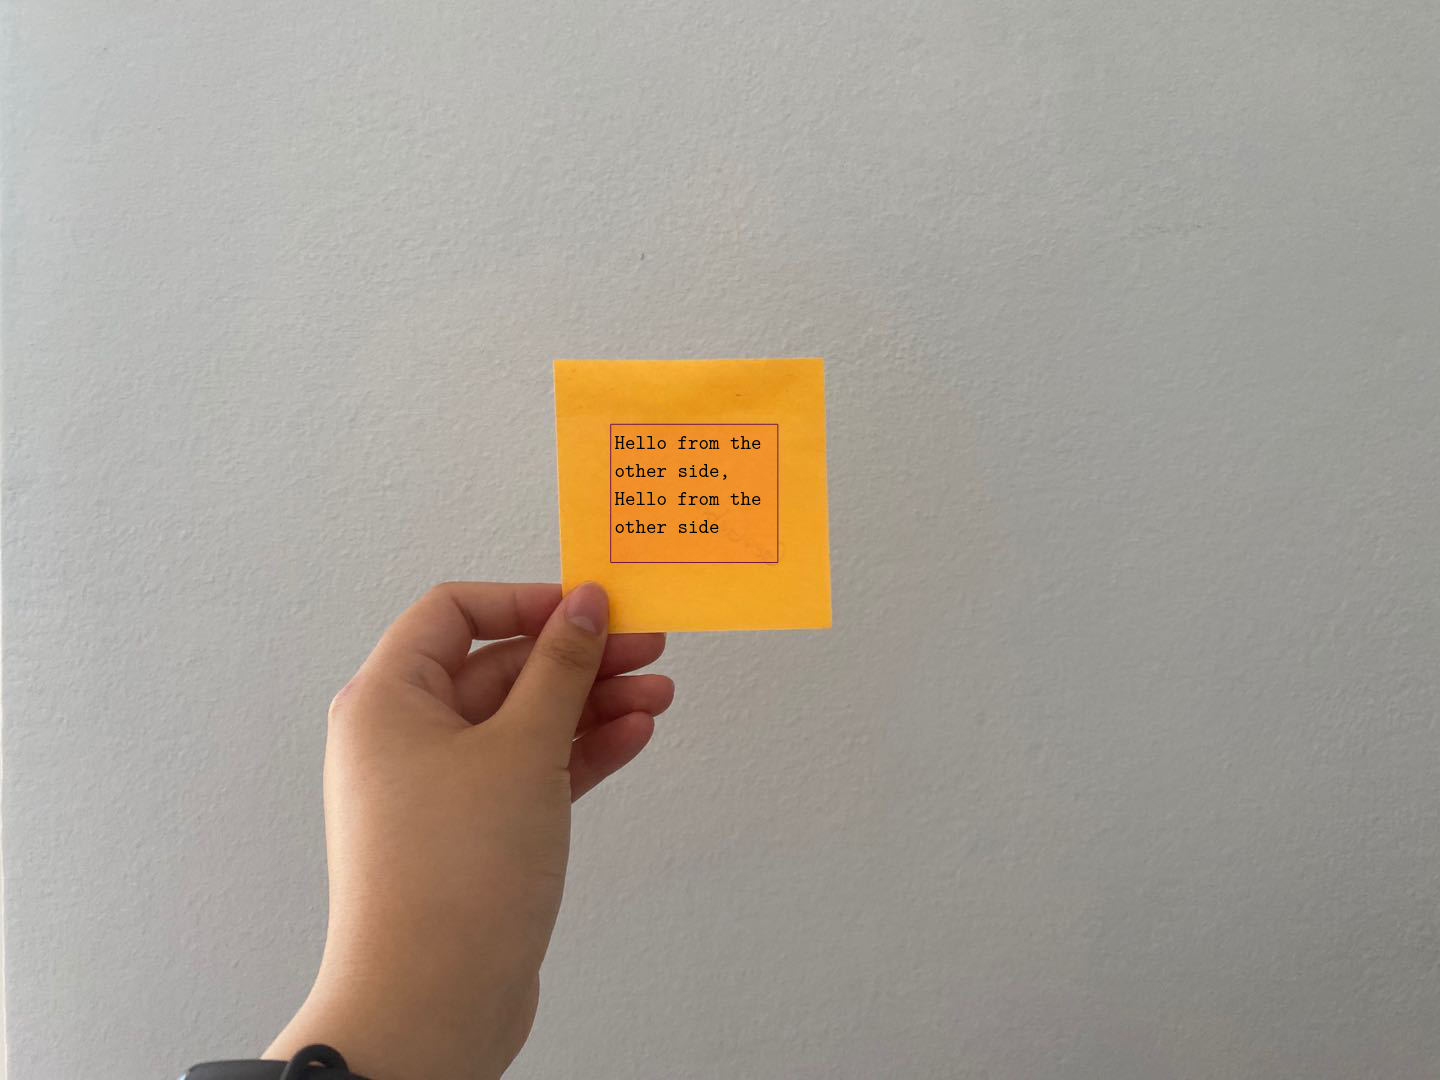
\includegraphics[width=.9\textwidth]{test.png}
\caption{Saved image with auto-adjusted text on it}
\end{figure}
\end{itemize}


\chapter{Flowchart}

\noindent Flowchart of the logic process of displaying text is attached as below.  \\ \par
\begin{figure}[h!]
\centering
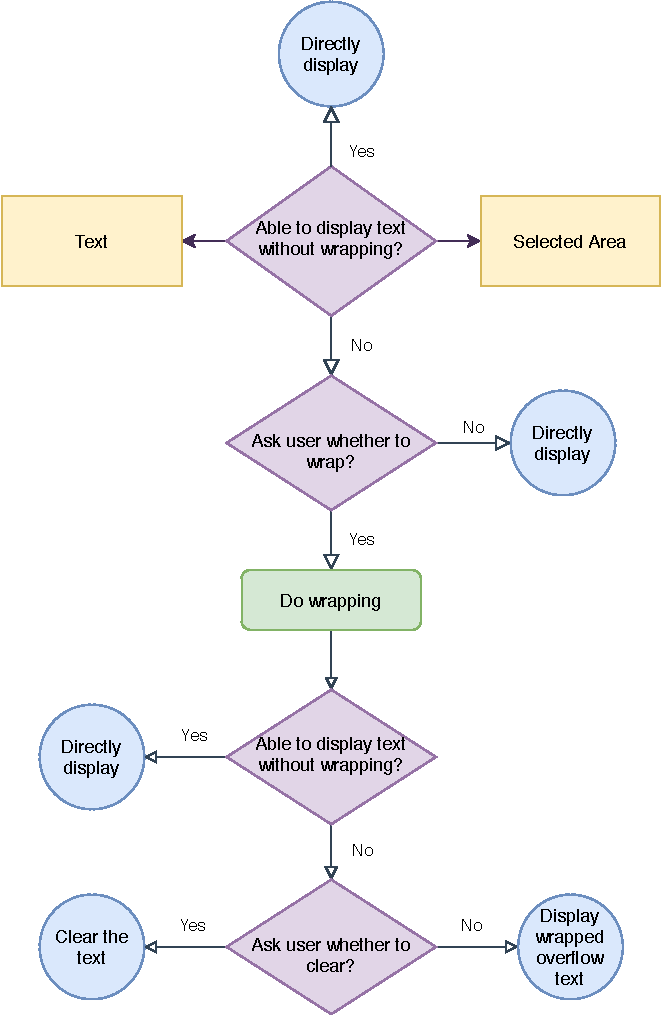
\includegraphics[width=.7\textwidth]{project_flowchart.pdf}
\caption{Flowchart of process of displaying text}
\end{figure}
\chapter{Text Adjuster}
\section{Project Structure}

\noindent A graphical user interfaces (GUI) for auto-adjusting text to mouse selected area inside of an image using PyQt5 has been successfully developed in this project.    \\ \par

\begin{figure}[h!]
\centering
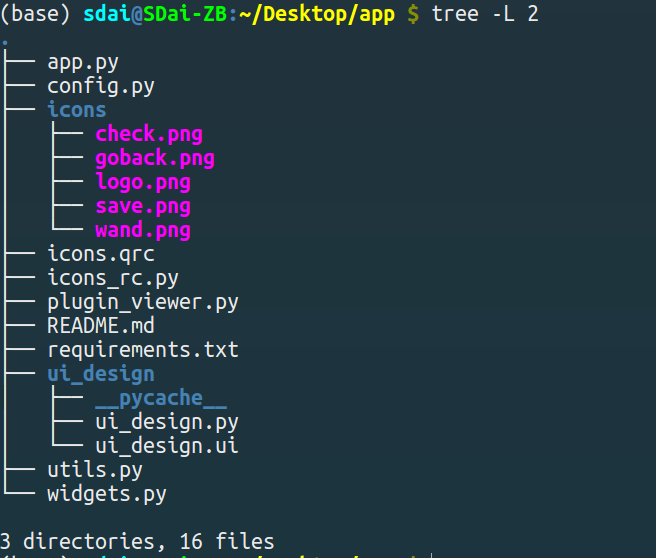
\includegraphics[width=.69\textwidth]{structure.png}
\caption{The project structure in level 2}
\end{figure}


\noindent The project folder is divided as:
\begin{itemize}
\item \textbf{app.py} executive file to run the text adjuster
\item \textbf{config.py} config file for saving information of the app and the default directory path image loading from
\item \textbf{icon} folder for storing icons used in the mainwindow
\item \textbf{icons.qrc and icons{\_}rc.py} icon related script auto-generated by \textit{the Resource Compiler for PyQt5 (Qt v5.13.0)}
\item \textbf{plugin{\_}viewer.py} general setting relates to the viewer, including the wheel event and mouse event setup for selecting text area in image.
\item \textbf{README.md} instruction for using the app
\item \textbf{requirement.txt} environment requirement
\item \textbf{ui{\_}design} folder for storing the design of the mainwindow from Qt Creator
\item \textbf{utils.py} some util functions for message boxes and load directory set
\item \textbf{widgets.py} main script with handlers for choosing images, input texts, position storing, and decide whether break line
\end{itemize}


\section{Code}
\noindent The scripts being used in this project has been attached as below. \\ \par

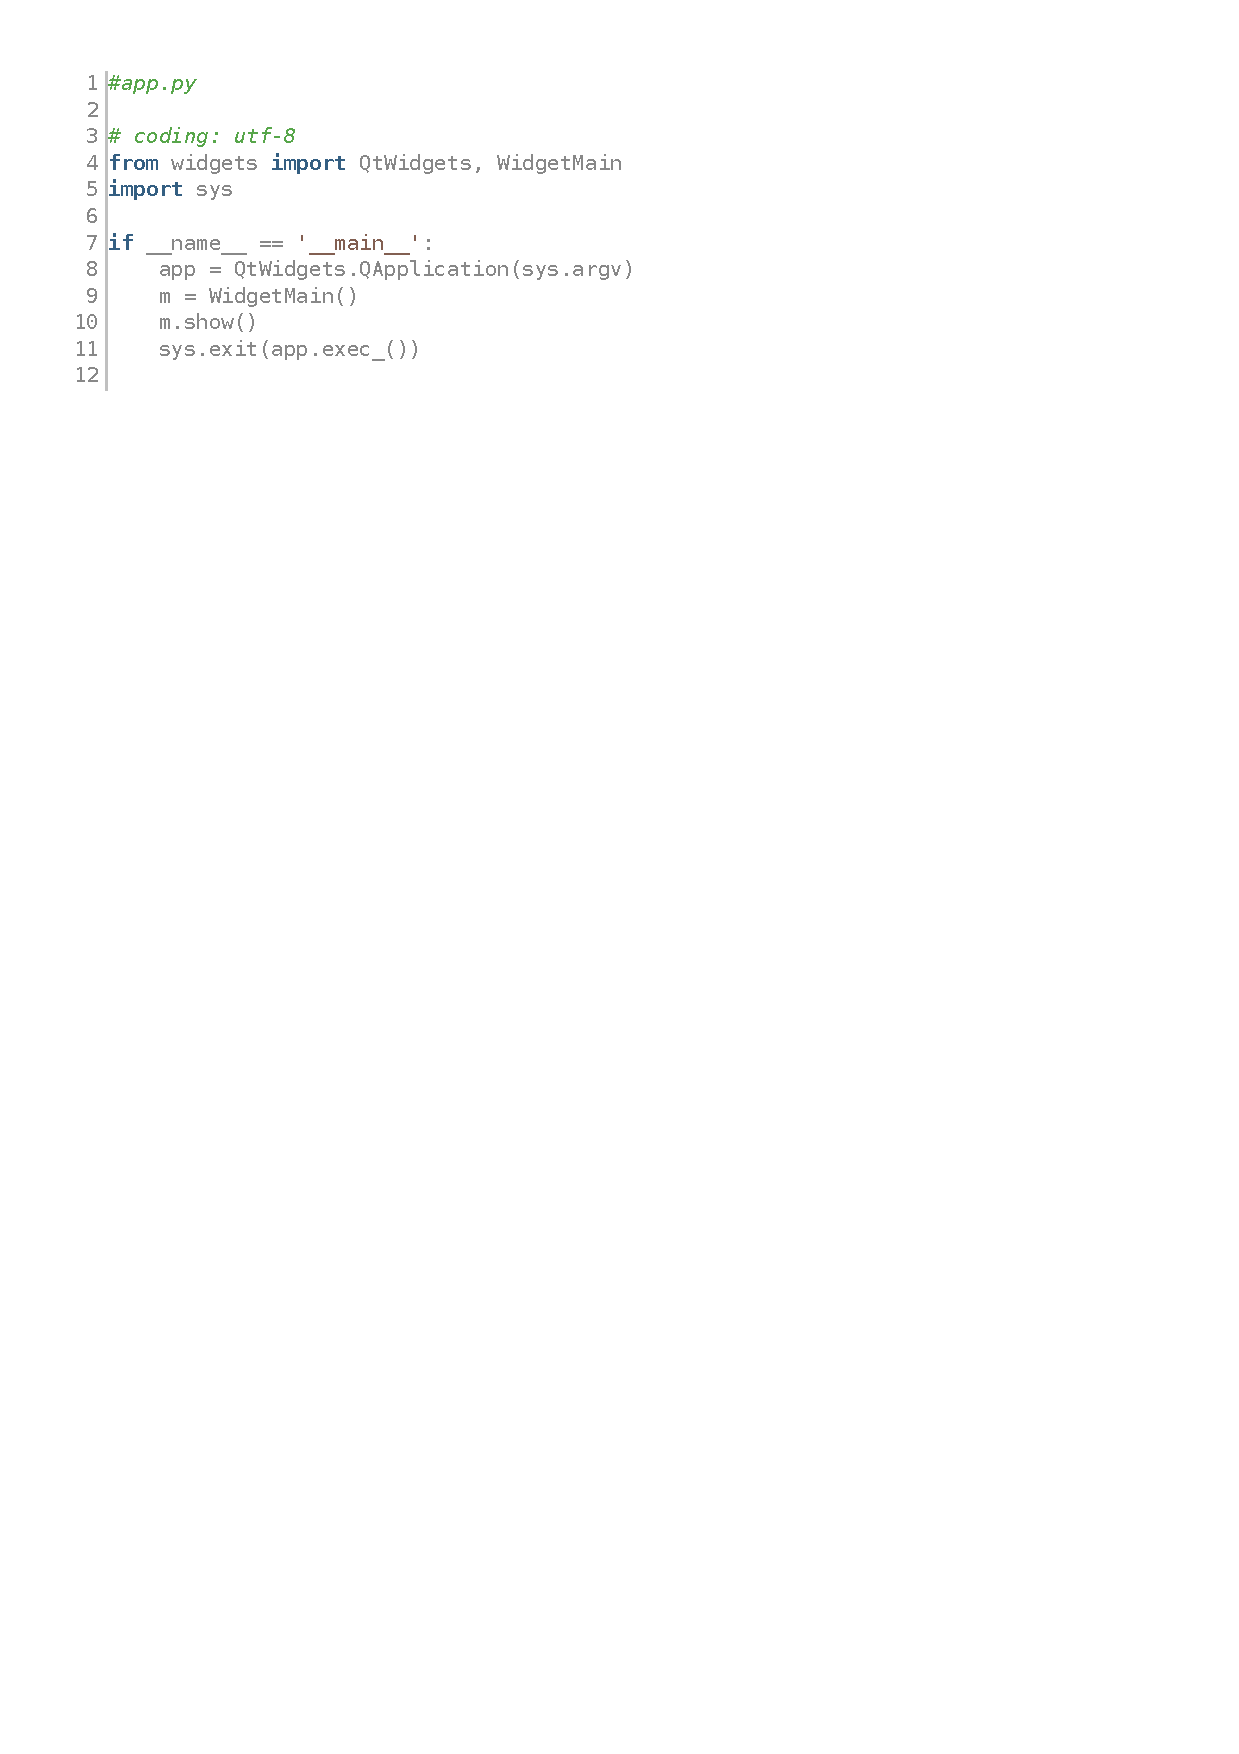
\includepdf[pages=-,pagecommand={},delta=3mm 3mm, frame = true, width=\textwidth]{app.pdf}
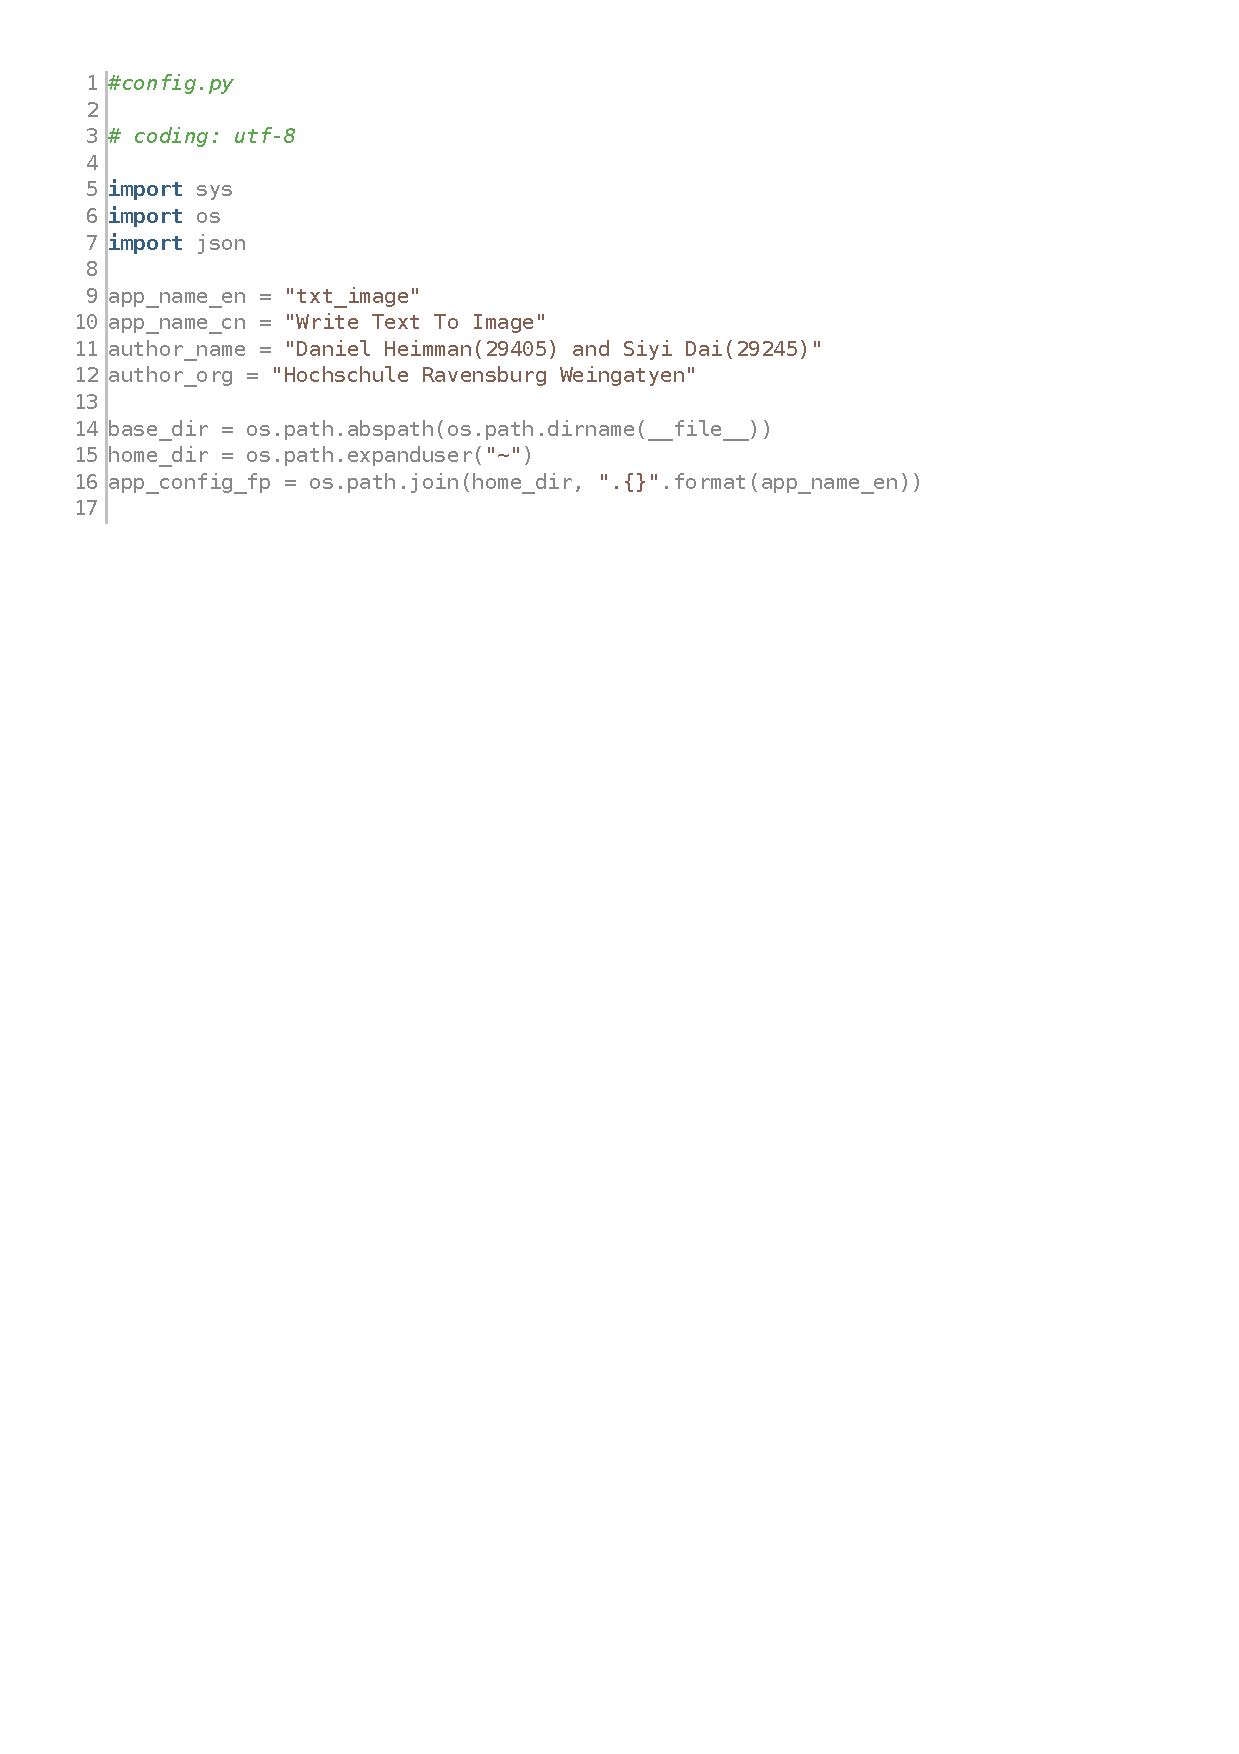
\includepdf[pages=-,pagecommand={},delta=3mm 3mm, frame = true, width=\textwidth]{config.pdf}
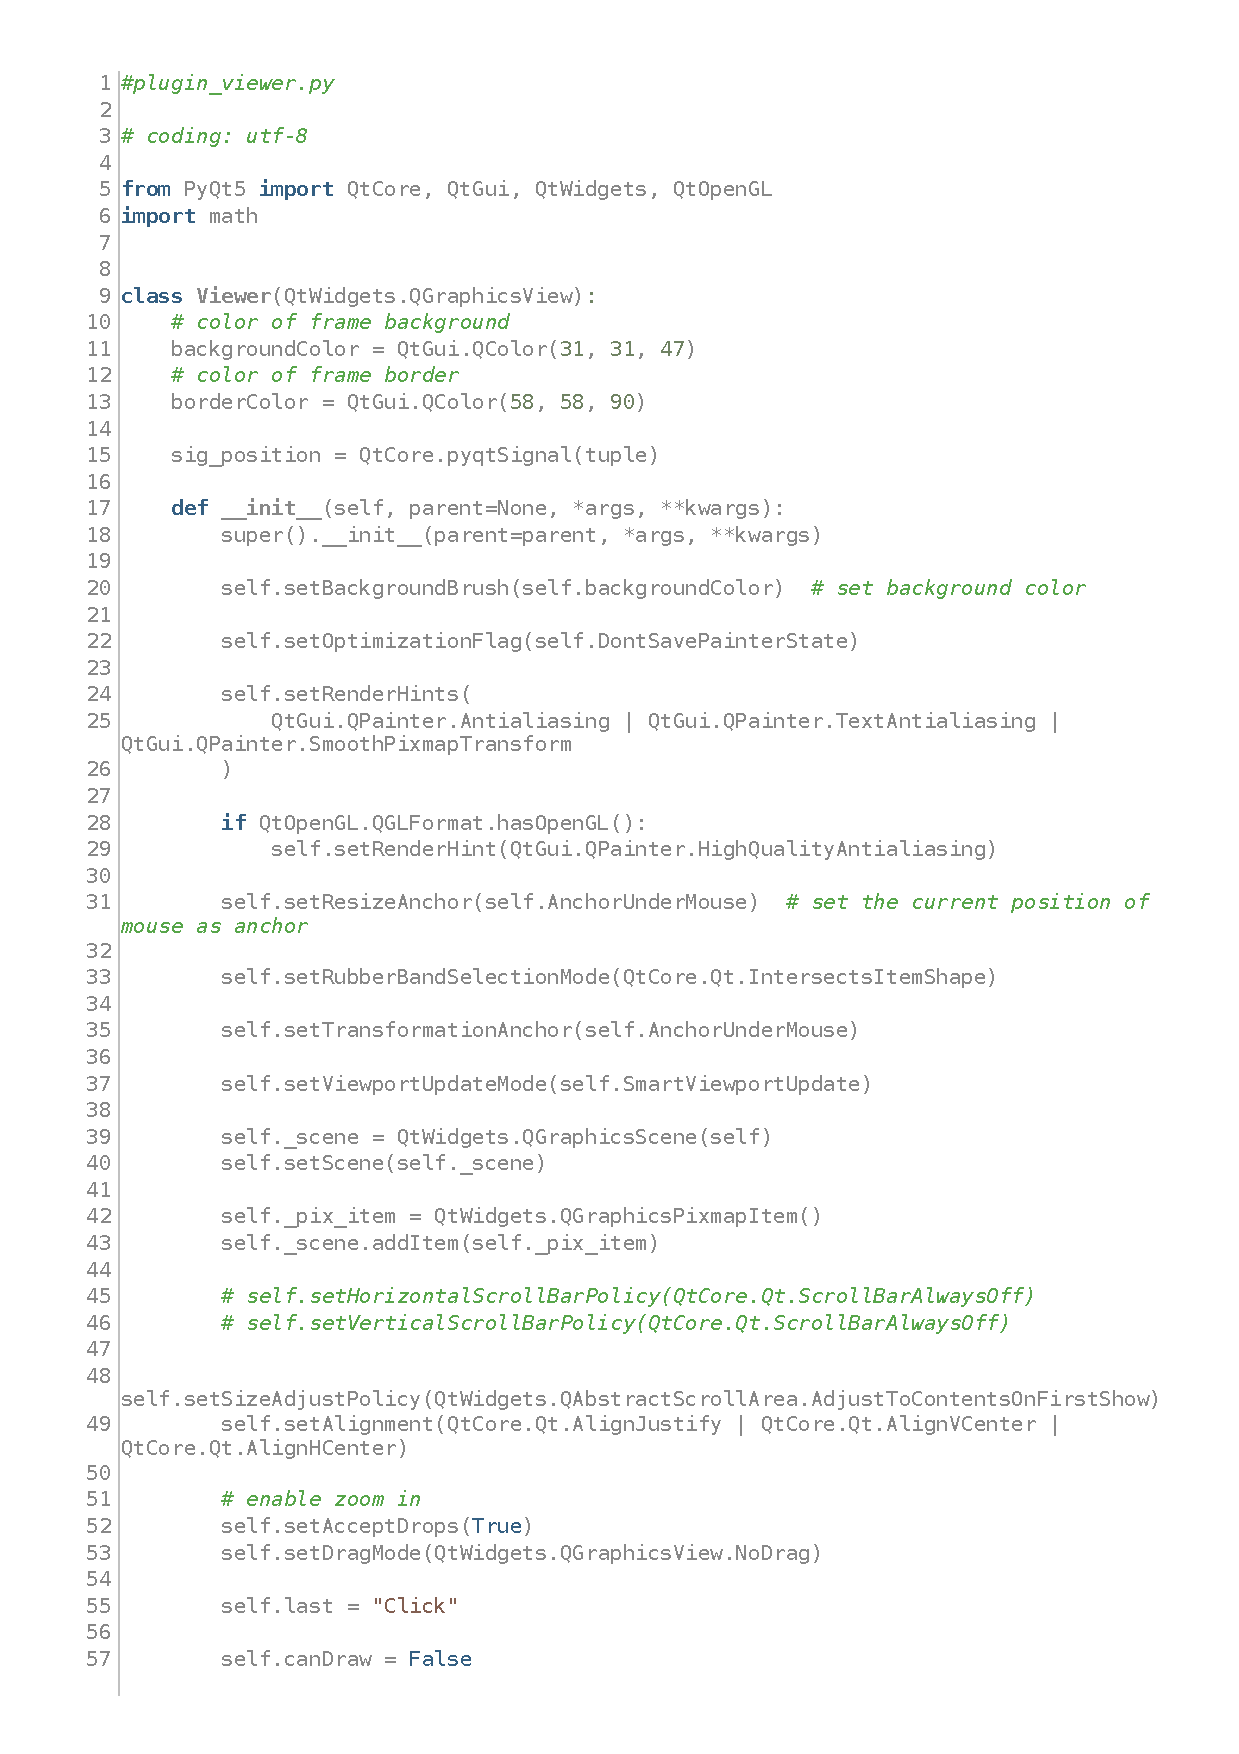
\includepdf[pages=-,pagecommand={},delta=3mm 3mm, frame = true, width=\textwidth]{plugin_viewer.pdf}
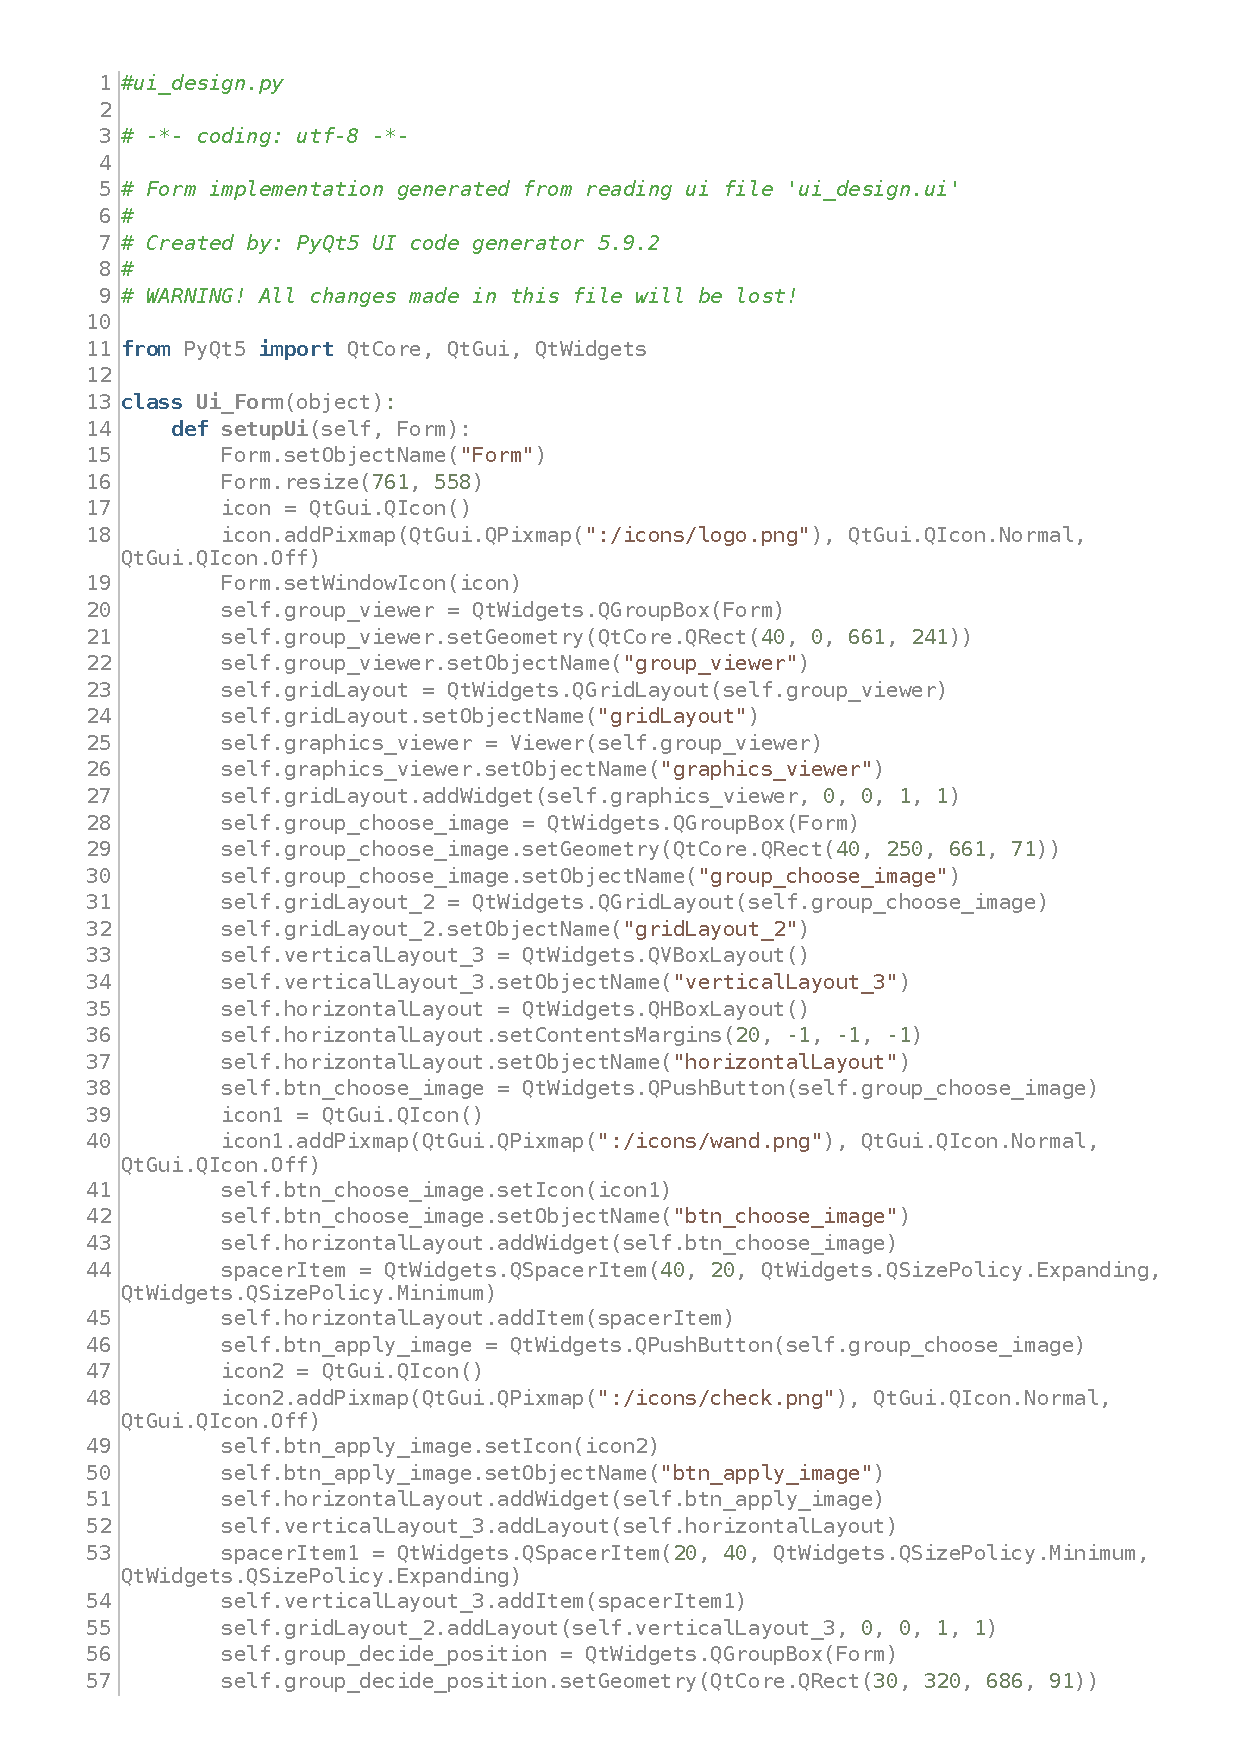
\includepdf[pages=-,pagecommand={},delta=3mm 3mm, frame = true, width=\textwidth]{design.pdf}
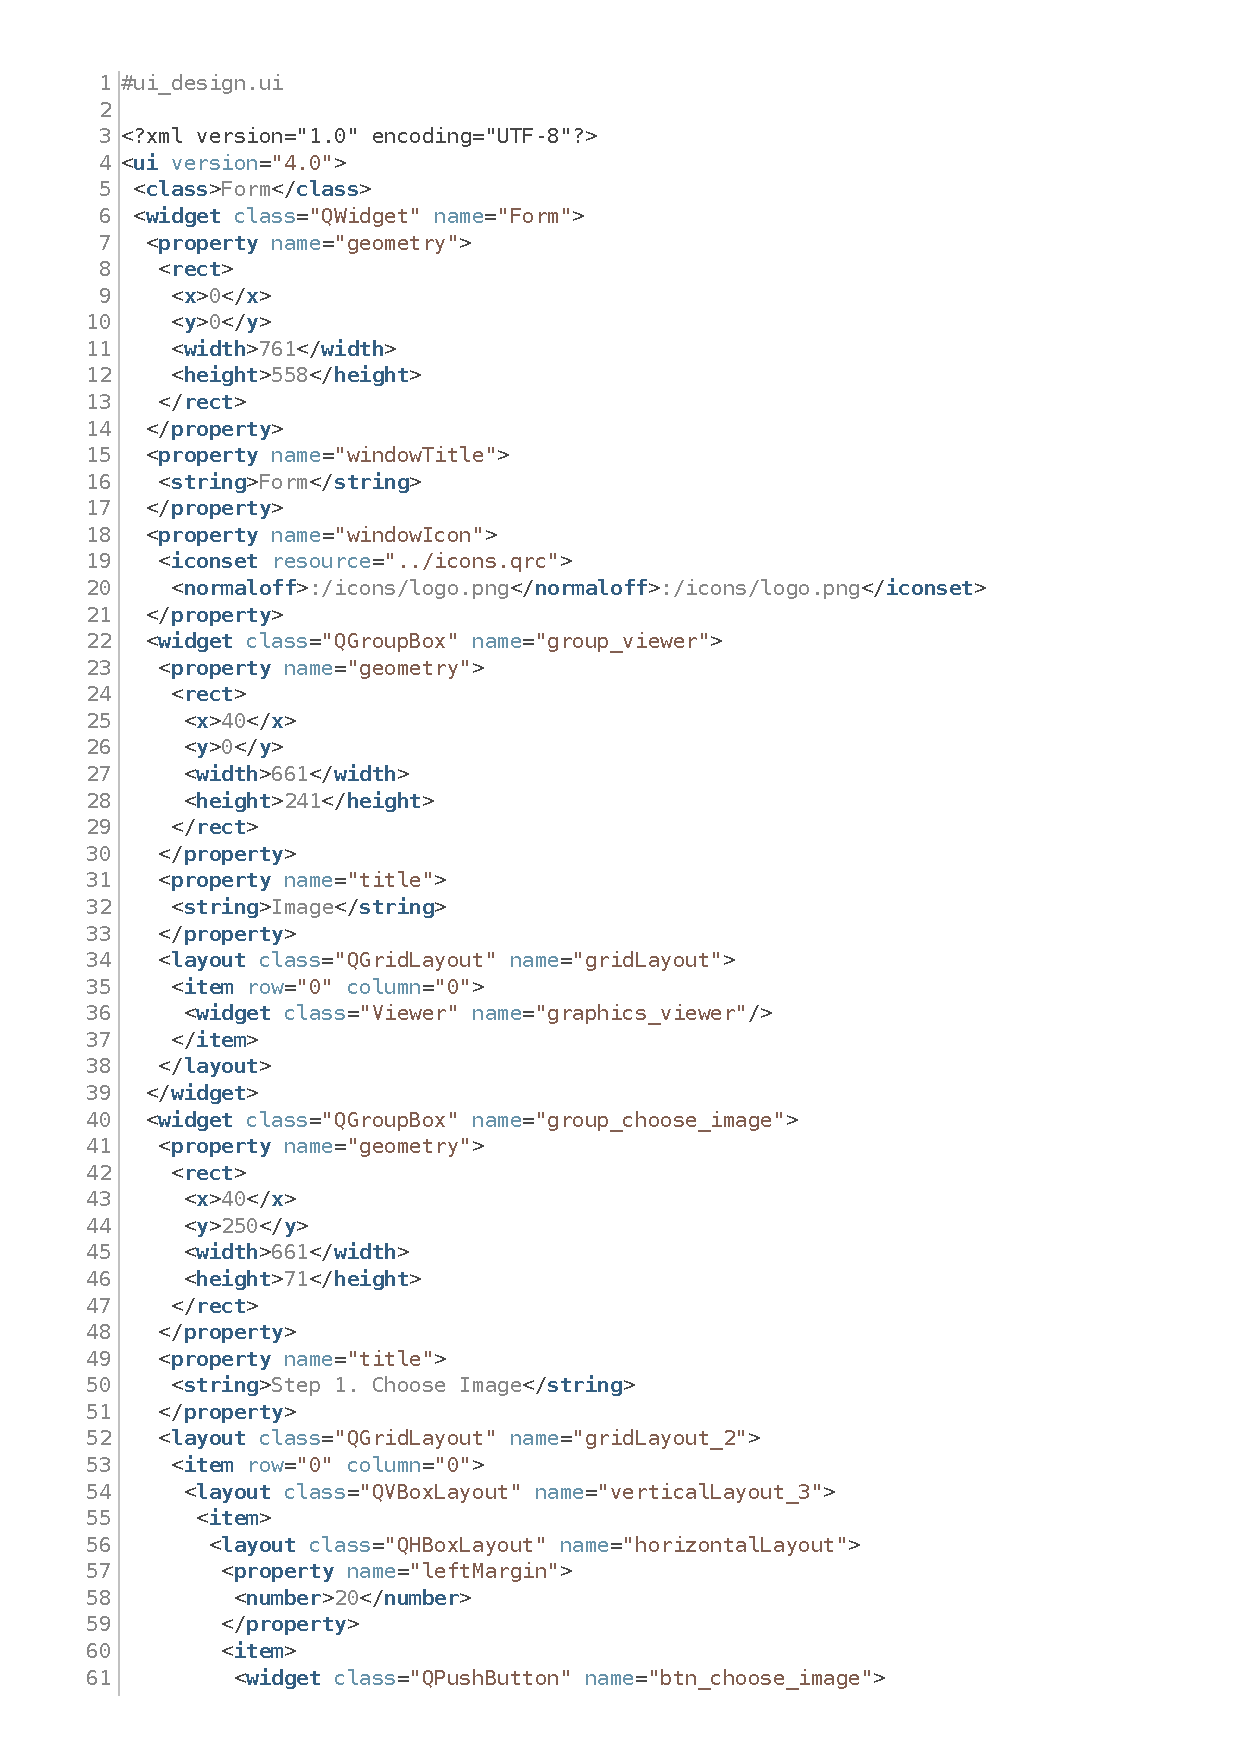
\includepdf[pages=-,pagecommand={},delta=3mm 3mm, frame = true, width=\textwidth]{ui_design.pdf}
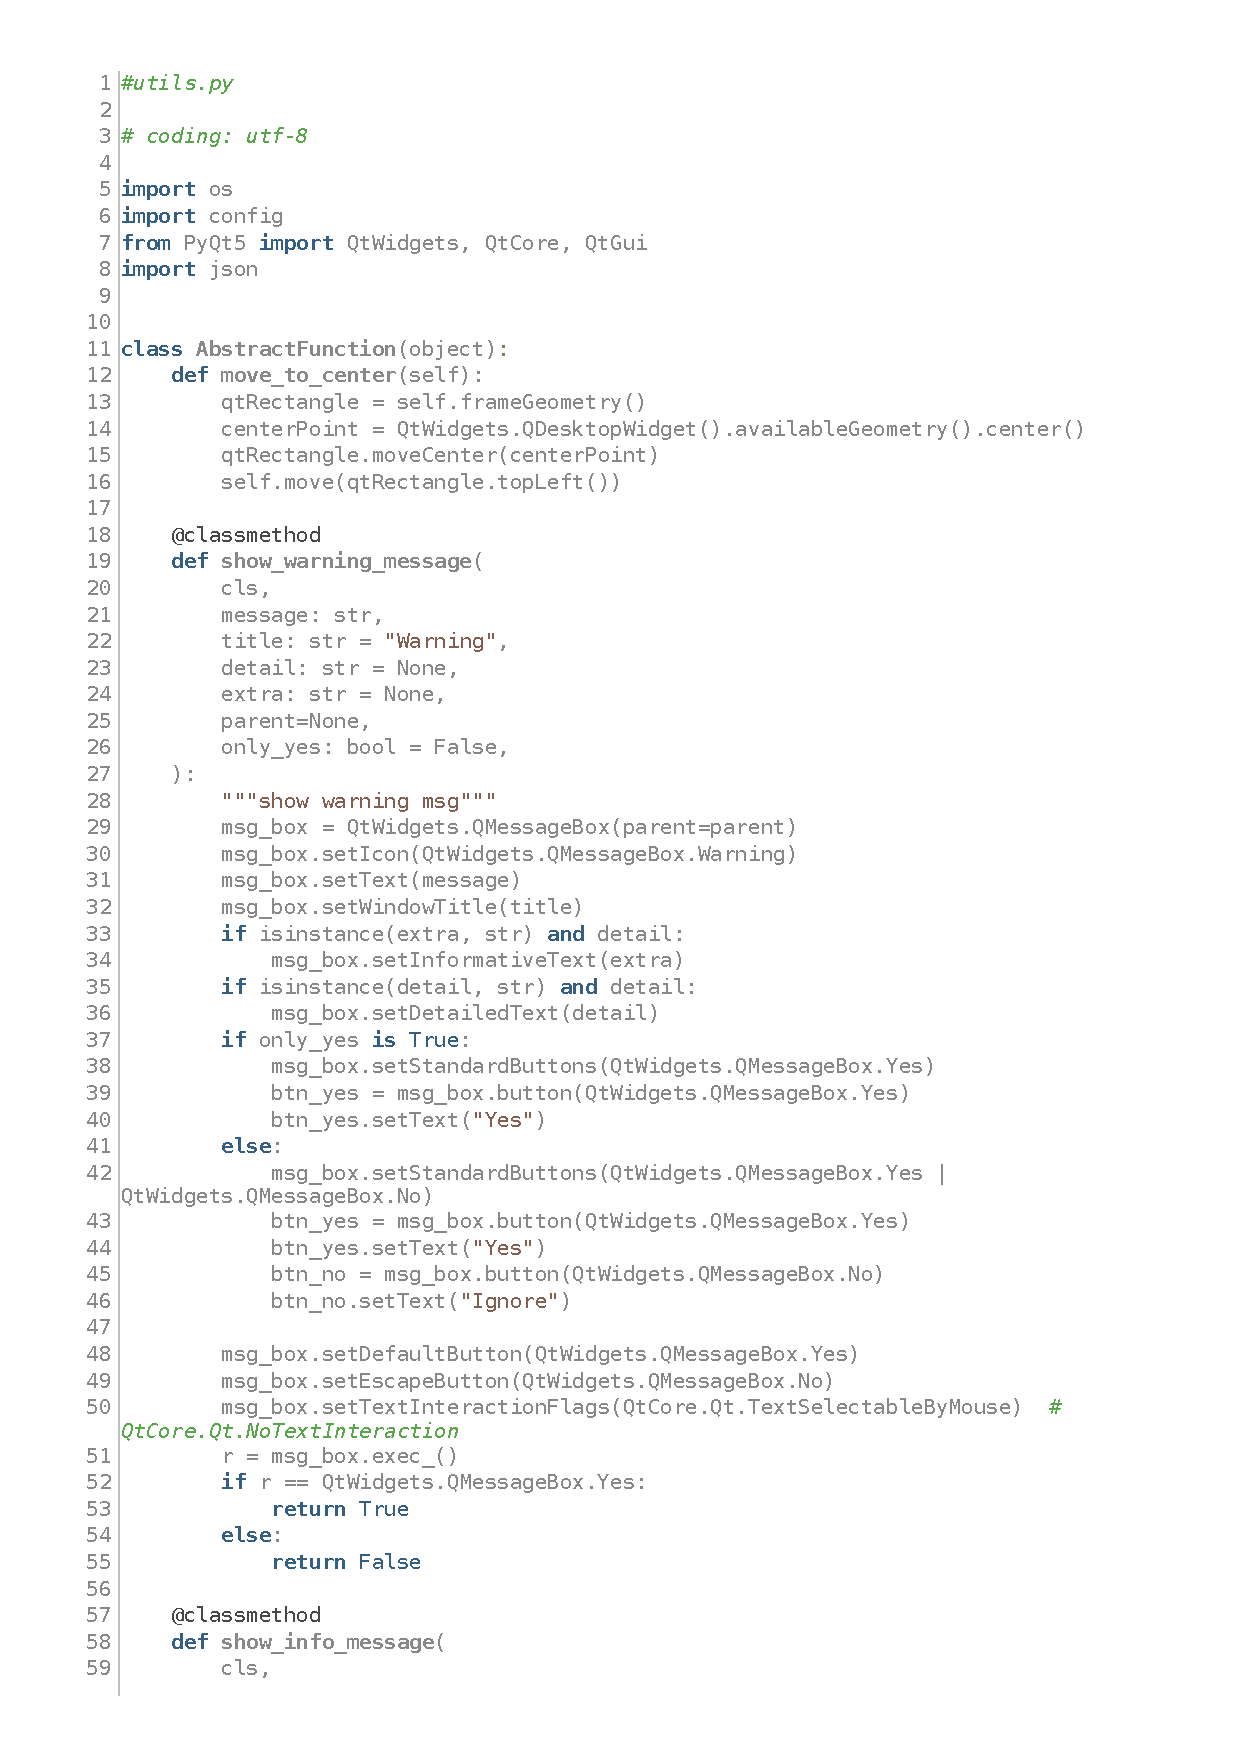
\includepdf[pages=-,pagecommand={},delta=3mm 3mm, frame = true, width=\textwidth]{utils.pdf}
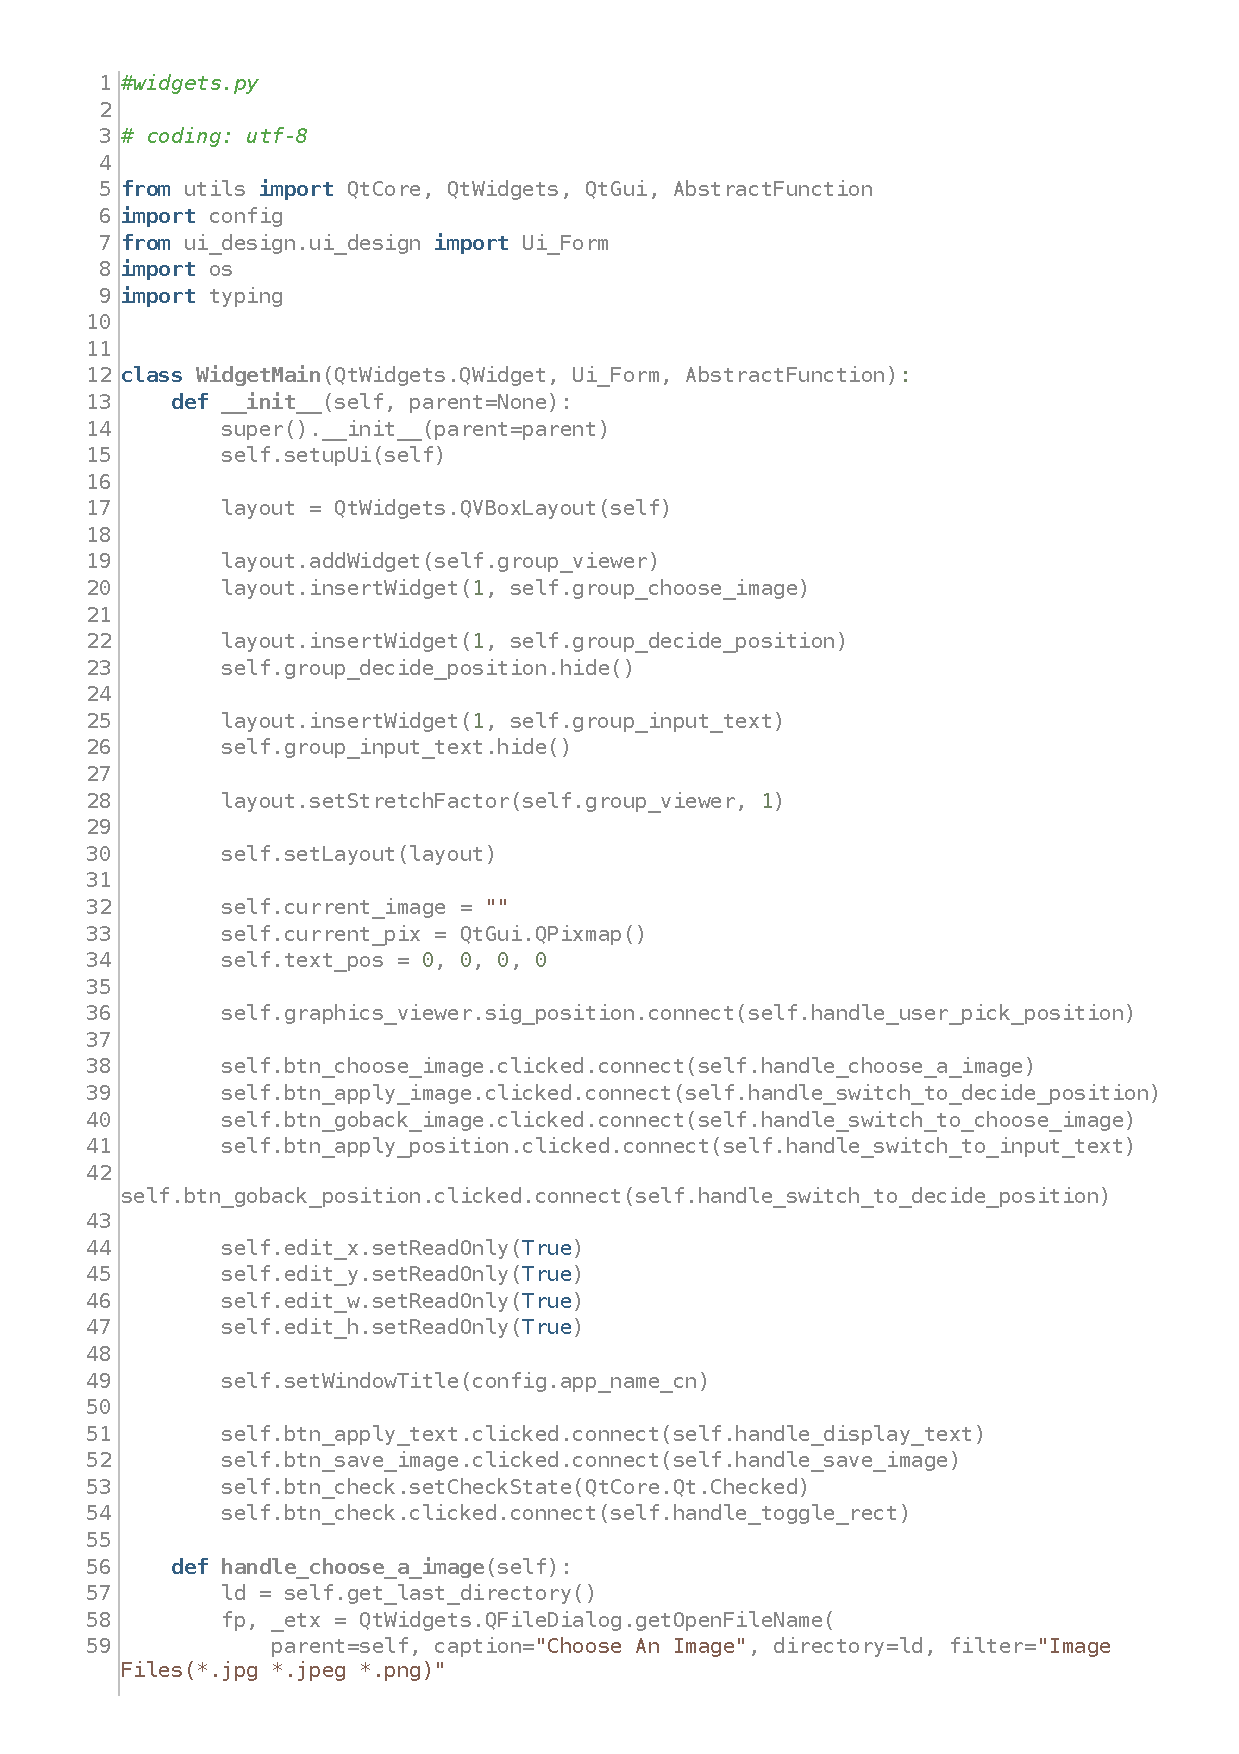
\includepdf[pages=-,pagecommand={},delta=3mm 3mm, frame = true, width=\textwidth]{widgets.pdf}
\newpage
% Here is the Bibliography of this document:
\begin{thebibliography}{1}

\bibitem{GUI}
\begin{flushleft}
Wikipedia - GUI, \url{https://en.wikipedia.org/wiki/Graphical_user_interface}
\end{flushleft} 

\bibitem{Qt}
\begin{flushleft}
Wikipedia - Qt (software), \newline \url{https://en.wikipedia.org/wiki/Qt_(software)}
\end{flushleft}

\bibitem{Qt Creator}
\begin{flushleft}
Wikipedia - Qt Creator, \newline \url{https://en.wikipedia.org/wiki/Qt_Creator}
\end{flushleft}

\bibitem{pyqt5}
\begin{flushleft}
Python - Introduction to PyQt5, \newline \url{https://www.geeksforgeeks.org/python-introduction-to-pyqt5/}
\end{flushleft}

\bibitem{Visual Studio Code}
\begin{flushleft}
Wikipedia - Visual Studio Code, \newline \url{
https://en.wikipedia.org/wiki/Visual_Studio_Code}
\end{flushleft}


\end{thebibliography}
\end{document}


